\documentclass[tikz,border=8pt]{standalone}
\usepackage{amsmath}
\usetikzlibrary{arrows.meta}
\usetikzlibrary{external}

% -------------------------------------------------
% Custom PGF/TikZ shape based on the supplied path
% -------------------------------------------------
\makeatletter
\pgfdeclareshape{wing}{
	
	% Standard anchors
	\savedanchor\centerpoint{\pgfpoint{0}{0}}
	
	\anchor{center}{\centerpoint}
	\anchor{north}{\pgfpoint{0}{1.7cm}}
	\anchor{south}{\pgfpoint{0}{-1.5cm}}
	\anchor{west}{\pgfpoint{-8cm}{0}}
	\anchor{east}{\pgfpoint{0}{0}}
	
	% Recommended text box
	\foregroundpath{
		% Scale down to resemble original drawing
		\pgftransformscale{0.5}
		
		\pgfpathmoveto{\pgfpoint{0cm}{0cm}}
		
		\pgfpathcurveto
		{\pgfpoint{-1.8cm}{0.9cm}}
		{\pgfpoint{-5.5cm}{1.7cm}}
		{\pgfpoint{-8cm}{0.25cm}}
		
		\pgfpathcurveto
		{\pgfpoint{-9cm}{-0.35cm}}
		{\pgfpoint{-8.2cm}{-1.5cm}}
		{\pgfpoint{-6.2cm}{-1.05cm}}
		
		\pgfpathcurveto
		{\pgfpoint{-3.8cm}{-0.55cm}}
		{\pgfpoint{-1.4cm}{0.2cm}}
		{\pgfpoint{0cm}{0cm}}
		
		\pgfpathclose
		
		\pgfsetlinewidth{0.8pt}
		\pgfsetstrokecolor{blue}
		\pgfusepath{draw}
	}
}
\makeatother

\tikzexternalenable

\begin{document}
	
	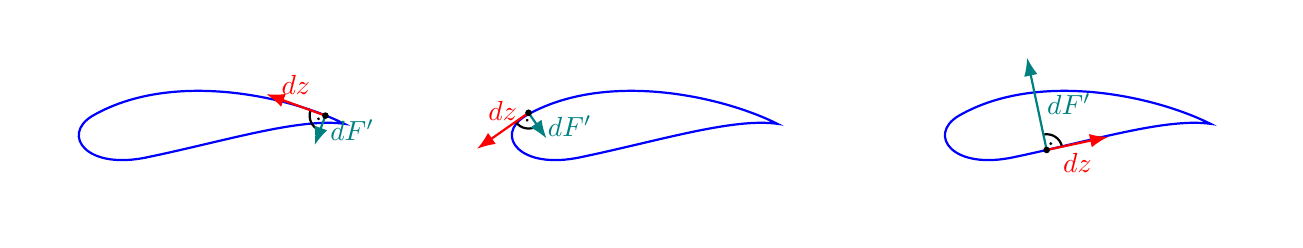
\begin{tikzpicture}[>=Latex]
		
		%--------------------------------------------------
		% Left figure
		%--------------------------------------------------
		\begin{scope}[xshift=0cm, scale=0.4]
			\coordinate (P) at (-0.6,0.26);
			\draw[white, very thick] (-10,-3) rectangle (2,3);
			\node[shape=wing, scale=0.8] at (0,0) {};
			
			\begin{scope}[rotate=-20]
				\fill (P)+(-0.17,-0.17) circle (0.05);
				
				\draw[thick]
				(P)+(-0.5,0)
				arc[start angle=180,end angle=270,radius=0.5];
				
				\draw[->, thick, red]
				(P) -- node[midway, above] {$dz$} +(180:2);
				
				\draw[->, thick, teal]
				(P) -- node[midway, right] {$dF'$} +(270:1);
			\end{scope}
			
			\fill (P) circle (3pt);
		\end{scope}
		
		%--------------------------------------------------
		% Middle figure
		%--------------------------------------------------
		\begin{scope}[xshift=5.5cm, scale=0.4]
			\coordinate (P) at (-7.9,0.35);
			\draw[white, very thick] (-10,-3) rectangle (2,3);
			\node[shape=wing, scale=0.8] at (0,0) {};
			
			\begin{scope}[rotate=35]
				\fill (P)+(-0.17,-0.17) circle (0.05);
				
				\draw[thick]
				(P)+(-0.5,0)
				arc[start angle=180,end angle=270,radius=0.5];
				
				\draw[->, thick, red]
				(P) -- node[midway, above] {$dz$} +(180:2);
				
				\draw[->, thick, teal]
				(P) -- node[midway, right] {$dF'$} +(270:1);
			\end{scope}
			
			\fill (P) circle (3pt);
		\end{scope}
		
		%--------------------------------------------------
		% Right figure
		%--------------------------------------------------
		\begin{scope}[xshift=11cm, scale=0.4]
			\coordinate (P) at (-5.2,-0.83);
			\draw[white, very thick] (-10,-3) rectangle (2,3);
			\node[shape=wing, scale=0.8] at (0,0) {};
			
			\begin{scope}[rotate=192]
				\fill (P)+(-0.17,-0.17) circle (0.05);
				
				\draw[thick]
				(P)+(-0.5,0)
				arc[start angle=180,end angle=270,radius=0.5];
				
				\draw[->, thick, red]
				(P) -- node[midway, below] {$dz$} +(180:2);
				
				\draw[->, thick, teal]
				(P) -- node[midway, right] {$dF'$} +(270:3);
			\end{scope}
			
			\fill (P) circle (3pt);
		\end{scope}
		
	\end{tikzpicture}
	
\end{document}